\chapter{Theorie des semileptonischen Zerfalles}

\section{Qualitative Beschreibung}

Das Feynman-Diagramm in führender Ordnung des untersuchten Zerfalles ist in Abbildung \ref{fig:feynman1} dargestellt.

\todo{Sich für den schönsten Feynmangraphen entscheiden}
\begin{figure}
  \centering
  \begin{tikzpicture}
  \begin{feynman}
    \vertex (a1) {\(b\)};
    \vertex[right=1cm of a1] (a2);
    \vertex[right=1cm of a2] (a3);
    %\vertex[right=1cm of a3] (a4) {\(b\)};
    \vertex[right=1cm of a3, label=125:\(V_{cb}\)] (a5);
    \vertex[right=2cm of a5] (a6) {\(c\)};

    \vertex[below=2em of a1] (b1) {\(\overline q\)};
    \vertex[right=1cm of b1] (b2);
    \vertex[right=1cm of b2] (b3);
    %\vertex[right=1cm of b3] (b4) {\(\overline d\)};
    \vertex[below=2em of a6] (b5) {\(\overline q\)};

    \vertex[above=of a6] (c1) {\(\overline \nu_l\)};
    \vertex[above=2em of c1] (c3) {\(l\)};
    \vertex at ($(c1)!0.5!(c3) - (1cm, 0)$) (c2);

    \diagram* {
      {[edges=fermion]
        (b5) -- (b1)
        (a1) -- (a5) -- (a6)
        %(b5) -- (b4) -- (b3) -- (a3) -- (a4) -- (a5) -- (a6),
      },


      (c1) -- [fermion, out=180, in=-45] (c2) -- [fermion, out=45, in=180] (c3),
      (a5) -- [boson, edge label=\(W^{-}\)] (c2),
    };

    \draw [decoration={brace}, decorate] (b1.south west) -- (a1.north west)
          node [pos=0.5, left] {\(\overline B\)};
    %\draw [decoration={brace}, decorate] (c3.north east) -- (c1.south east)
    %      node [pos=0.5, right] {\(\pi^{-}\)};
    \draw [decoration={brace}, decorate] (a6.north east) -- (b5.south east)
          node [pos=0.5, right] {\(D\)};
  \end{feynman}
  \end{tikzpicture}
  \caption{Feynman-Diagramm des semileptonischen Zerfalles $B \to D l \overline \nu_l$ in führender Ordnung.}
  \label{fig:feynman1}
\end{figure}

Im Eingangszustand befindet sich ein $\overline B$-Meson, welches aus einem $b$-Quark und einem leichten Antiquark $\overline q$ ($ \overline q = \overline u, \overline d)$ besteht.
Die schwache Wechselwirkung führt zu einer Umwandlung des beteiligten $b$-Quarks in ein $c$-Quark unter Emission eines $W^{-}$-Bosons. Dieses $W^{-}$-Boson ist ein virtuelles Teilchen und zerfällt direkt weiter in ein Lepton $l$ und das dazugehörige Antineutrino $\overline \nu_l$.
Zusätzlich ist bei diesem Prozess zu beachten, dass die schwache Wechselwirkung nicht an die Masseneigenzustände der Quarks koppelt.
Die korrekten Eigenzustände der Quarks $d'$, $s'$ und $b'$ für die schwache Wechselwirkung sind stattdessen Linearkombinationen der Masseneigenzustände von $d$, $s$ und $b$. Sie ergeben sich somit durch eine Rotation der ursprünglichen Eigenzustände.
Diese Rotation wird durch die unitäre CKM-Matrix beschrieben.
Der für den betrachteten Zerfall relevante Parameter $\lvert V_{cb} \rvert$ beträgt \cite{Bigi2017441}
\begin{equation}
  \lvert V_{cb} \rvert = \SI{40.49+-0.97e-3}{}
.
\end{equation}

\begin{figure}
  \centering
  \begin{tikzpicture}
  \begin{feynman}
    \vertex (a1) {\(b\)};
    \vertex[right=1cm of a1] (a2);
    \vertex[right=1cm of a2] (a3);
    %\vertex[right=1cm of a3] (a4) {\(b\)};
    \vertex[right=1cm of a3, label=125:\(V_{cb}\)] (a5);
    \vertex[right=2cm of a5] (a6) {\(c\)};

    \vertex[below=4em of a1] (b1) {\(\overline q\)};
    \vertex[right=1cm of b1] (b2);
    \vertex[right=1cm of b2] (b3);
    \vertex[below=2em of a3] (g1);
    \vertex[left=1.8cm of a6] (g2);
    \vertex[right=1cm of b2] (g5);
    \vertex[left=0.5cm of a6] (g6);
    \vertex[right=1.5cm of g1] (g3);
    \vertex[right=0.8cm of g3] (g4);
    %\vertex[right=1cm of b3] (b4) {\(\overline d\)};
    \vertex[below=4em of a6] (b5) {\(\overline q\)};

    \vertex[above=of a6] (c1) {\(\overline \nu_l\)};
    \vertex[above=2em of c1] (c3) {\(l\)};
    \vertex at ($(c1)!0.5!(c3) - (1cm, 0)$) (c2);

    \diagram* {
      {[edges=fermion]
        (b5) -- (b1)
        (a1) -- (a5) -- (a6)
        %(b5) -- (b4) -- (b3) -- (a3) -- (a4) -- (a5) -- (a6),
      },


      (c1) -- [fermion, out=180, in=-45] (c2) -- [fermion, out=45, in=180] (c3),
      (a5) -- [boson, edge label=\(W^{-}\)] (c2),

      (a2) -- [gluon] (g1)
      (b2) -- [gluon] (g1)
      (g1) -- [gluon] (g2)
      (g5) -- [gluon] (g3)
      (g3) -- [fermion, half left] (g4)
      (g4) -- [fermion, half left] (g3)
      (g4) -- [gluon] (g6)

    };

    \draw [decoration={brace}, decorate] (b1.south west) -- (a1.north west)
          node [pos=0.5, left] {\(\overline B\)};
    %\draw [decoration={brace}, decorate] (c3.north east) -- (c1.south east)
    %      node [pos=0.5, right] {\(\pi^{-}\)};
    \draw [decoration={brace}, decorate] (a6.north east) -- (b5.south east)
          node [pos=0.5, right] {\(D\)};
  \end{feynman}
  \end{tikzpicture}
  \caption{Exemplarisches Feynman-Diagramm des semileptonischen Zerfalles $B \to D l \overline \nu_l$ unter Berücksichtigung der starken Wechselwirkung zwischen den beteiligten Quarks.}
  \label{fig:feynman2}
\end{figure}

Zusätzlich ist bei der Beschreibung des vorliegenden Zerfalles die starke Wechselwirkung zu berücksichtigen.
Sie führt, vermittelt durch den Austausch von Gluonen, zur Bindung zwischen dem als Zuschauerquark agierenden Antiquark sowie dem schwach wechselwirkenden Quark.
Aufgrund des nicht-pertubativen Verhaltens der starken Wechselwirkung bei großen Abständen werden auch die Beiträge der Feynman-Diagramme höherer Ordnung, wie in Abbildung \ref{fig:feynman2} exemplarisch dargestellt, relevant.
Primäres Ziel der Formfaktoren ist es, diese Effekte bei der Berechnung der Zerfallsraten quantitativ zu Berücksichtigen.

\section{Parametrisierung des Matrixelementes durch Formfaktoren}

Das Matrixelement $M$ des Zerfalles lässt sich allgemein als \todo{Abstände zwischen den Bra/Kets optimieren}
\begin{align*}
  M = \bra{D \, l \, \overline{\nu_l}} H \ket{ \overline{B} }
\end{align*}
mit dem Hamiltonian $H$ des Zerfalles beschreiben.
Es ist außerdem möglich, das Matrixelement in einen hadronischen Anteil mit dem Hamiltonian $H_\text{had}$ und einen leptonischen Anteil mit dem Hamiltonian $H_\text{lep}$ zu faktorisieren, so dass sich das Matrixelement
\begin{align*}
  M = \bra{ l \, \overline{\nu_l}} H_\text{lep} \ket{0}  \bra{D} H_\text{had}  \ket{ \overline{B} }
\end{align*}
ergibt.
Der hadronische Faktor wird durch einen V-A-Strom
\begin{align*}
  \bra{D} H_\text{had}  \ket{ \overline{B} } = \bra{D} \, \overline{c} \gamma_\mu (1 - \gamma_5) b \, \ket{ \overline{B} } = \bra{D} \underbrace{\overline{c} \gamma_\mu b }_{= V_\mu} \ket{\overline{B} } - \bra{D} \, \underbrace{ \overline{c} \gamma_\mu \gamma_5 b}_{= A_\mu}\, \ket{ \overline{B} }
\end{align*}
beschrieben, wobei $b$ hier der Spinor des $b$-Quarks und $\overline{c}$ der adjungierte Spinor des $c$-Quarks ist.
Die Bezeichnungen $V_\mu$ und $A_\mu$ für die Ströme drücken aus, dass sich unter Parität $V_\mu = \overline{c} \gamma_\mu b$ wie ein Vektor und $A_\mu = \overline{c} \gamma_\mu \gamma_5 b$ wie ein Axialvektor transformiert.
Da die hier betrachteten Mesonen pseudoskalare Größen sind, stehen zur Parametrisierung des Matrixelementes als dynamische Variablen der Viererimpuls des $\overline{B}$-Mesons $p^B$ sowie der Viererimpuls des $D$-Mesons $p^D$ zur Verfügung.
Zusätzlich lässt sich hieraus der Lorentz-Skalar
\begin{equation}
  q^2 = (p^B-p^D)^2
\end{equation}
konstruieren, welcher den Impulsübertrag zwischen den Mesonen ausdrückt.

Sowohl die dynamische Variable $p^B$ als auch $p^D$ transformieren sich wie Vektoren.
Aus diesen Größen lässt sich jedoch kein Ausdruck konstruieren, der sich wie ein Axialvektor transformiert.
Da die Quantenchromodynamik die Parität erhält, folgt hieraus direkt, dass der axiale Anteil des hadonischen Matrixelementes verschwinden muss:
\begin{align*}
  \bra{D} A_\mu \ket{\overline{B}} = 0.
\end{align*}
Somit verbleibt der vektorielle Anteil des hadronischen Matrixelementes, welcher durch
\begin{equation}
  \bra{D} V_\mu \ket{\overline{B}} = f_+(q^2)(p^B + p^D)_\mu + f_{-}(q^2)(p^B - p^D)_\mu
\end{equation}
mit den Formfaktoren $f_+(q^2)$, $f_{-}(q^2)$ parametrisiert wird.

Mithilfe dieser Parametrisierung kann, unter Nutzung der Feynmanregeln, die differentielle Zerfallsbreite für den betrachteten Zerfall berechnet werden.
Sie ergibt sich zu \cite{PhysRevD.94.094008}
\begin{equation}
  \label{eqn:difzb}
  \frac{\mathrm{d} \Gamma}{\mathrm{d} q^2} \left(\overline{B} \to D l \overline{\nu_l} \right) = \frac{\eta_\text{EW}^2 G_\text{F}^2 \lvert V_{cb} \rvert^2 m_B \sqrt{\lambda} }{192 \pi^3} \left( 1 - \frac{m_l^2}{q^2} \right)^2 \left( c_+^l f_+(q^2)^2 + c_0^l f_0(q^2)^2 \right)
\end{equation}
mit den Abkürzungen
\begin{align*}
  c_+^l &= \frac{\lambda}{m_B^4} \left( 1 + \frac{m_l^2}{2 q^2} \right) & c_0^l &= \left(1 - \frac{m_D^2}{m_B^2} \right)^2 \frac{3 m_l^2}{2 q^2}
\end{align*}
sowie
\begin{align*}
  \lambda = (q^2 - m_B^2 - m_D^2)^2 - 4 m_B^2 m_D^2
\end{align*}
und
\begin{equation}
  \label{eqn:constraint}
  f_0(q^2) = f_+(q^2) + f_{-}(q^2) \frac{q^2}{m_B^2 - m_D^2}.
\end{equation}

\section{Kinematik des Zerfalles}

Aus der Viererimpulserhaltung $p^B = p^D + p^l + p^{\overline{\nu_l}}$ lassen sich Einschränkungen an den kinematisch erlaubten Bereich des Impulsübertrages $q^2$ stellen.
Diese Einschränkungen ergeben sich, wenn die beiden kinematischen Extremfälle betrachtet werden, welche jeweils in Abbildung \ref{fig:recoil} skizziert sind.
Es ergibt sich hieraus, dass der Impulsübertrag im Bereich
\begin{equation}
  m_l^2 \leq q^2 \leq (m_B - m_D)^2
  \label{eqn:kinematik}
\end{equation}
liegen kann.
\begin{figure}
  \centering
  \begin{subfigure}{0.48\textwidth}
    \centering
    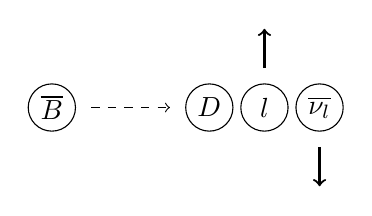
\begin{tikzpicture}
      \draw (0,0) circle [radius=0.3] node {$\overline{B}$};
      \draw[dashed, ->] (0.5, 0) -- (1.5, 0);
      \draw (2,0) circle [radius=0.3] node {$D$};
      \draw (2.7,0) circle [radius=0.3] node {$l$};
      \draw[thick, ->] (2.7, 0.5) -- (2.7, 1.0);
      \draw (3.4,0) circle [radius=0.3] node {$\overline{\nu_l}$};
      \draw[thick, ->] (3.4, -0.5) -- (3.4, -1.0);
    \end{tikzpicture}
    \caption{Kinematik bei $q_\text{max}^2 = (m_B - m_D)^2$.}
    \label{fig:recoil1}
  \end{subfigure}
  \begin{subfigure}{0.48\textwidth}
    \centering
    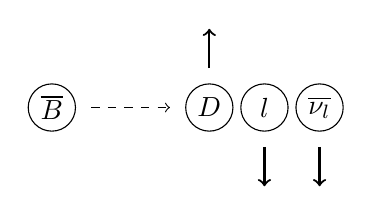
\begin{tikzpicture}
      \draw (0,0) circle [radius=0.3] node {$\overline{B}$};
      \draw[dashed, ->] (0.5, 0) -- (1.5, 0);
      \draw (2,0) circle [radius=0.3] node {$D$};
      \draw[thick, ->] (2, 0.5) -- (2, 1.0);
      \draw (2.7,0) circle [radius=0.3] node {$l$};
      \draw[thick, ->] (2.7, -0.5) -- (2.7, -1.0);
      \draw (3.4,0) circle [radius=0.3] node {$\overline{\nu_l}$};
      \draw[thick, ->] (3.4, -0.5) -- (3.4, -1.0);
    \end{tikzpicture}
    \caption{Kinematik bei $q_\text{min}^2 = m_l^2$.}
    \label{fig:recoil2}
  \end{subfigure}
  \caption{Kinematische Extremfälle beim Impulsübertrag.}
  \label{fig:recoil}
\end{figure}
\todo{Wirklich dieses Diagramm behalten? Und "zero-recoil"-Begriff bei a) einbringen?}

Für den Impulsübertrag $q^2$ werden häufig alternative Parametrisierungen verwendet.
Eine Möglichkeit stellt die $w$-Parametrisierung
\begin{equation}
  w(q^2) = \frac{m_B^2 + m_D^2 - q^2}{2 m_B m_D}
\end{equation}
dar, dessen Abhängigkeit von $q^2$ in Abbildung \ref{fig:w_param} dargestellt ist.
Hierbei wird der maximale Impulsübertrag $q_\text{max}^2$ auf $w=0$ abgebildet.

Eine weitere Parametrisierung, welche für den im folgenden Kapitel durchgeführten Fit der Formfaktoren von Bedeutung ist, findet sich in der Variable
\begin{equation}
  z(q^2) = \frac{\sqrt{w+1}-\sqrt{2}}{\sqrt{w+1}+\sqrt{2}}.
\end{equation}
Diese Parametrisierung von $q^2$ bildet den maximalen Impulsübertrag $q_\text{max}^2$ auf $z=0$ ab, wie in Abbildung \ref{fig:z_param} dargestellt ist.
Betrachtet man $z(q^2)$ zusätzlich außerhalb des kinematisch erlaubten Bereiches, so wird der Impulsübertrag, wie in Abbildung \ref{fig:z_kreis} dargestellt, auf die komplexe Ebene abgebildet.
Dabei bewegt sich $z$ auf einem Einheitshalbkreis in der oberen komplexen Halbebene, so dass $\lvert z \rvert \leq \num{1}$ immer erfüllt ist.
\begin{figure}
  \centering
  \includegraphics[width=0.9\textwidth]{pycode/plot_z_2.pdf}
  \caption{Abbildung von $q^2$ durch $z$ auf die komplexe Ebene. In grün wird der nach Gleichung \eqref{eqn:kinematik} kinematisch erlaubte Bereich dargestellt. Die gestrichelte rote Line verdeutlicht den unphysikalischen Bereich negativer Impulsüberträge.}
  \label{fig:z_kreis}
\end{figure}

\begin{figure}
  \centering
  \begin{subfigure}{0.48\textwidth}
    \centering
    \includegraphics[width=\textwidth]{pycode/plot_w.pdf}
    \caption{Parametrisierung mit $w(q^2)$.}
    \label{fig:w_param}
  \end{subfigure}
  \begin{subfigure}{0.48\textwidth}
    \centering
    \includegraphics[width=\textwidth]{pycode/plot_z.pdf}
    \caption{Parametrisierung mit $z(q^2)$.}
    \label{fig:z_param}
  \end{subfigure}
  \caption{Parametrisierung des Impulsübertrages. Der im vorliegenden Zerfall erlaubte kinematische Bereich nach Gleichung \eqref{eqn:kinematik} wird durch den blauen Kasten verdeutlicht.}
\end{figure}
